
Using PhaZor, the six designs have been simulated, and the transmissions are normalised with respect to a reference waveguide. The results are shown in Fig. \ref{fig:simplots}.
\vspace{-0.1mm}
\begin{figure}[H]
\begin{subfigure}[h]{0.50\textwidth}
        \centering
        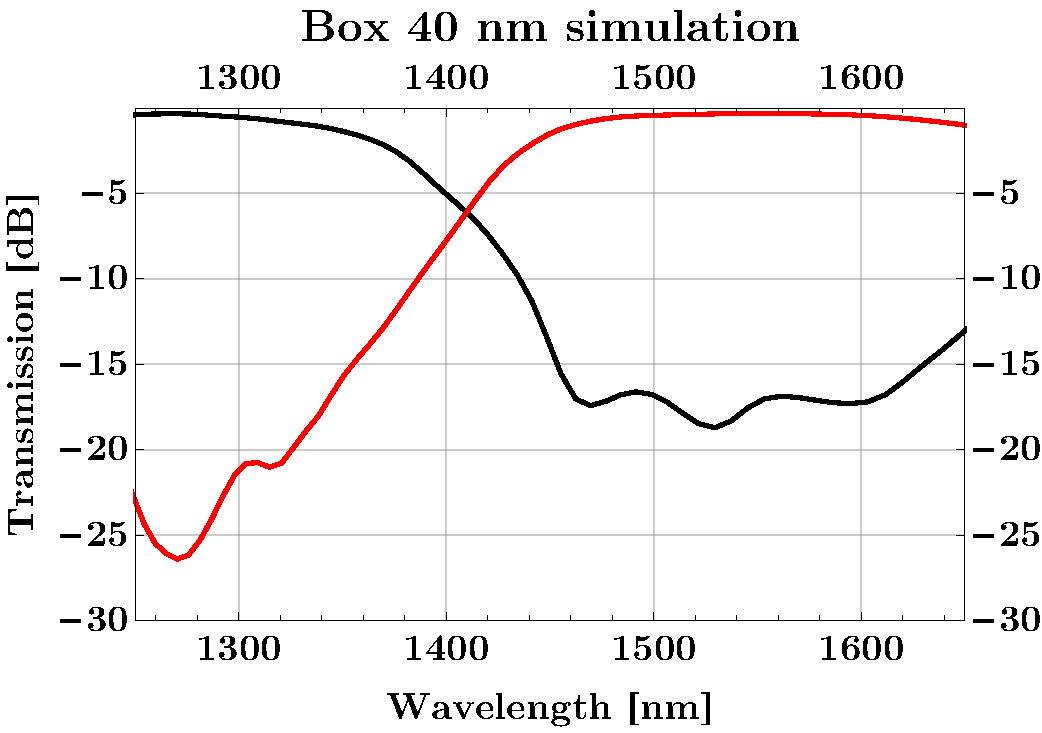
\includegraphics[width=1.0\textwidth]
        {fig/simplots/Kasse40nmsimplot.pdf}
        \caption{Simulated transmission through the box structure with feature size 40 nm.}
        \label{fig:transmissionkilde3_a}
    \end{subfigure}%
    ~ 
    \begin{subfigure}[h]{0.50\textwidth}
        \centering
        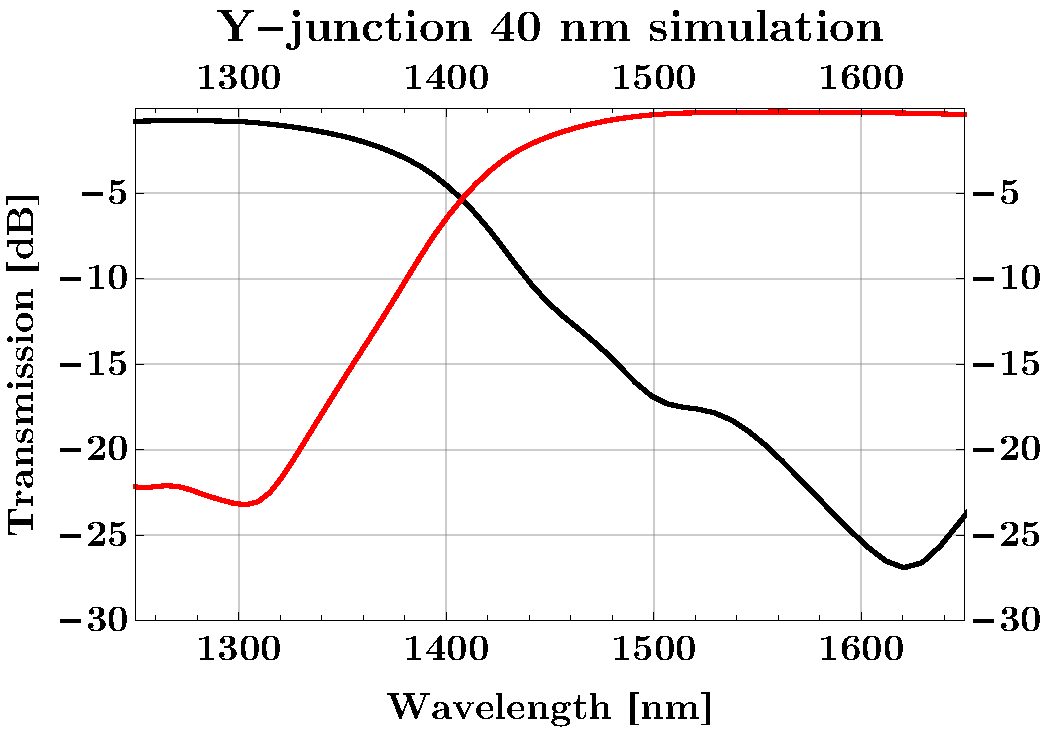
\includegraphics[width=1.0\textwidth]
        {fig/simplots/Yjunc40nmsimplot.pdf}
        \caption{Simulated transmission through the Y-junction structure with feature size 40 nm.}
    \end{subfigure}
    
    \vspace{5 mm}
    
    
    \begin{subfigure}[h]{0.50\textwidth}
        \centering
        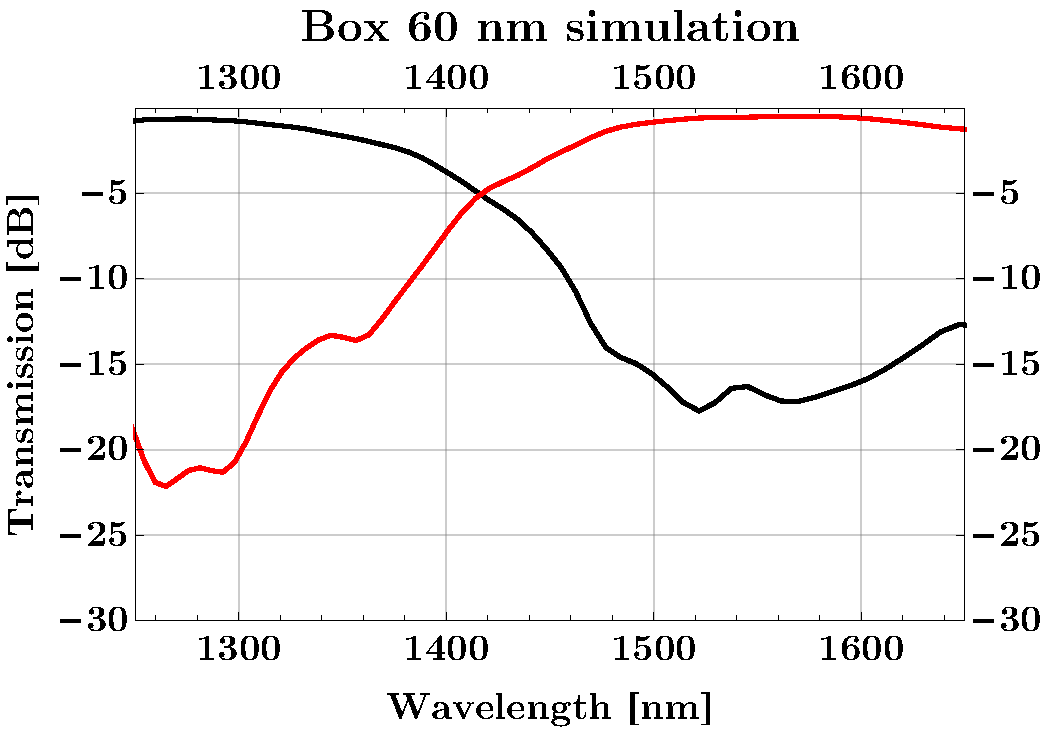
\includegraphics[width=1.0\textwidth]
        {fig/simplots/Kasse60nmsimplot.pdf}
        \caption{Simulated transmission through the box structure with feature size 60 nm.}
    \end{subfigure}%
    ~ 
    \begin{subfigure}[h]{0.50\textwidth}
        \centering
        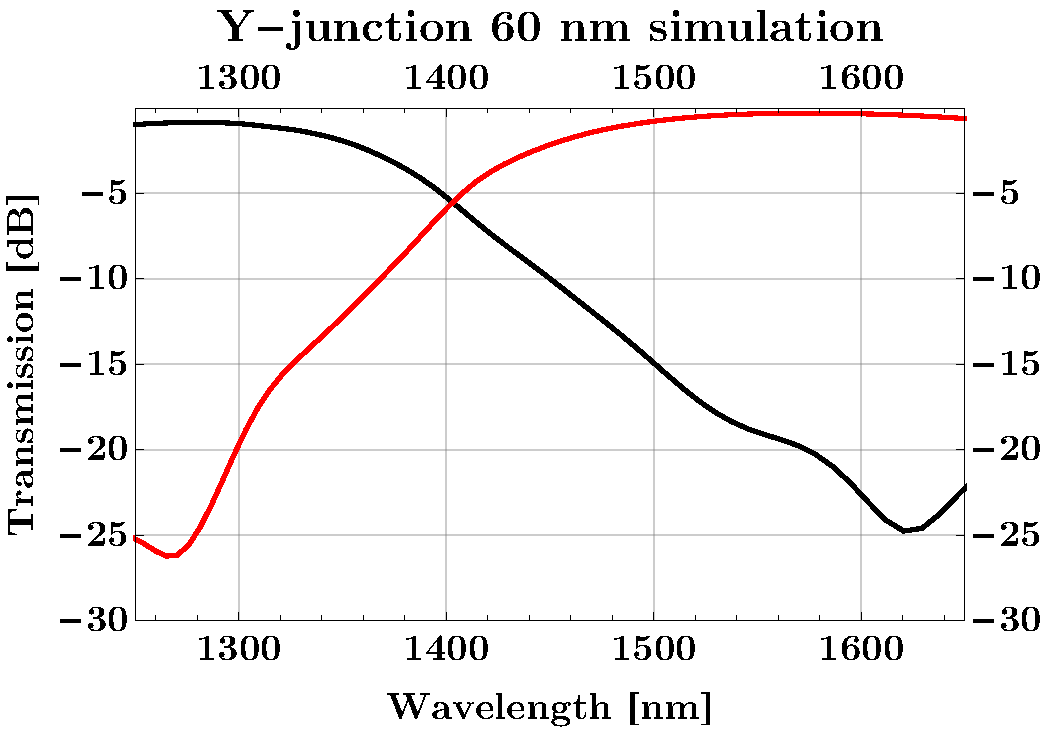
\includegraphics[width=1.0\textwidth]
        {fig/simplots/Yjunc60nmsimplot.pdf}
        \caption{Simulated transmission through the Y-junction structure with feature size 60 nm.}
    \end{subfigure}
    
    \vspace{5 mm}
    
    \begin{subfigure}[h]{0.5\textwidth}
        \centering
        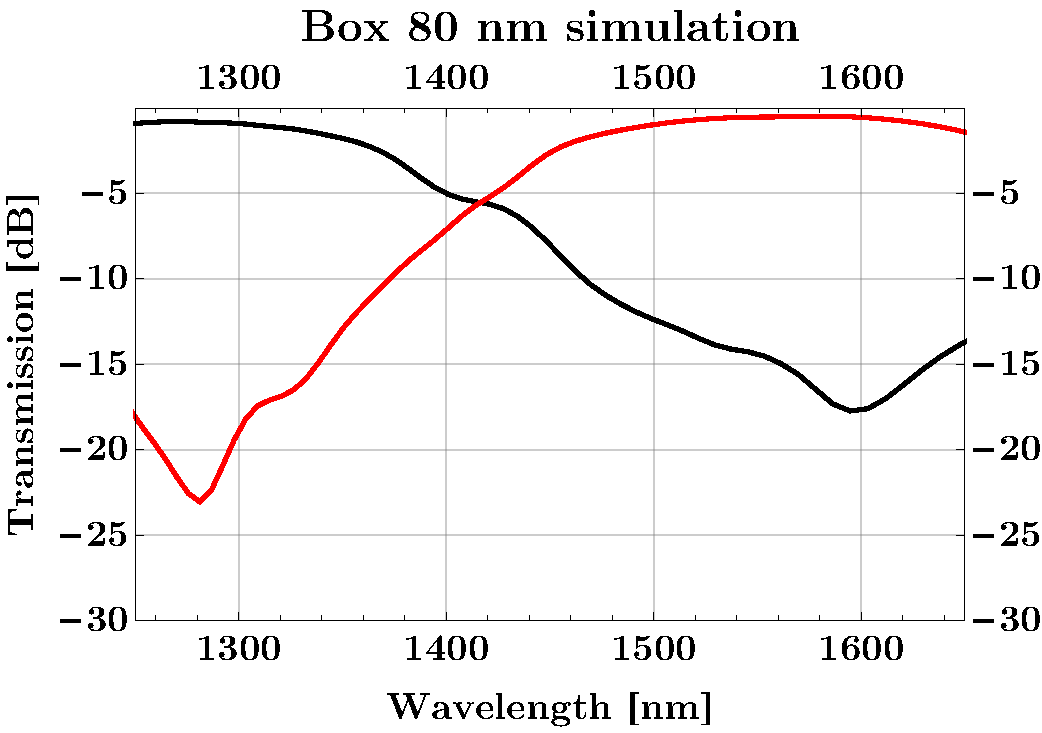
\includegraphics[width=1.0\textwidth]
        {fig/simplots/Kasse80nmsimplot.pdf}
        \caption{Simulated transmission through the box structure with feature size 80 nm.}
    \end{subfigure}%
    ~ 
    \begin{subfigure}[h]{0.50\textwidth}
        \centering
        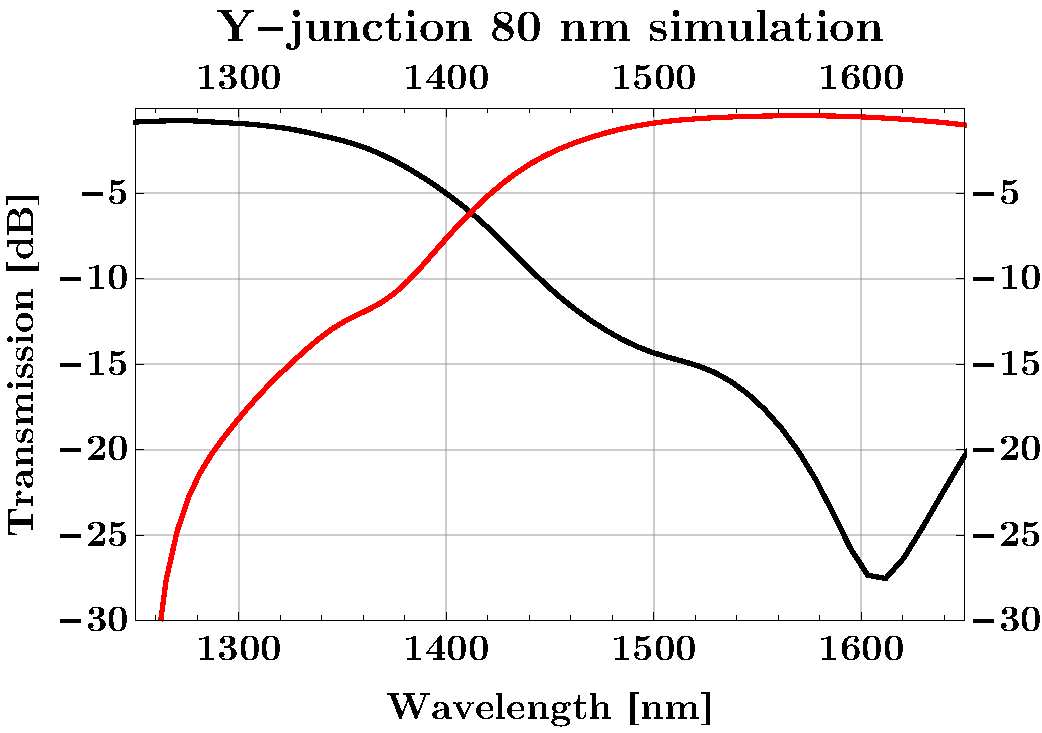
\includegraphics[width=1.0\textwidth]
        {fig/simplots/Yjunc80nmsimplot.pdf}
        \caption{Simulated transmission through the Y-junction structure with feature size 80 nm.}
    \end{subfigure}

    \caption{Simulation experiment results. Black: Upper output waveguide. Red: Lower output waveguide. Almost all designs have peak insertion losses at around $-0.5$ dB. For most structures, we see the intercept between the signal graphs at 1420-1422 nm wavelengths. Crosstalk is maximally around $-7$ dB, but much lower through most of the spectrum.}
   \label{fig:simplots}
    
\end{figure}

\newpage
